\documentclass[12pt, oneside]{article}

% Language setting
% Replace `english' with e.g. `spanish' to change the document language
\usepackage[english]{babel}

% Set page size and margins
% Replace `letterpaper' with `a4paper' for UK/EU standard size
\usepackage[letterpaper,top=2cm,bottom=2cm,left=3cm,right=3cm,marginparwidth=1.75cm]{geometry}

% Useful packages
\usepackage{amsmath}
\usepackage{graphicx}
\usepackage[colorlinks=true, allcolors=blue]{hyperref}
\usepackage{graphicx} % Required for inserting images
\usepackage{cite}
\usepackage{amsmath,amssymb,amsfonts}
\usepackage{algorithmic}
\usepackage{graphicx}
\usepackage{textcomp}
\usepackage{xcolor}
\usepackage{csquotes}
\usepackage{placeins}
\usepackage{etoolbox}
\usepackage{graphicx}
\usepackage{wrapfig}
\usepackage{subfigure}
\usepackage{subcaption}
\usepackage{IEEEtrantools}

\begin{document}

\begin{titlepage}
    \begin{center}
        \vspace*{1cm}
        {\huges
        \center{\huge{\textbf{Advanced Control and Dynamics}}}}
         \\
         \vspace{0.3cm}
         \large{Coursework Report}
         \vspace{0.5cm}
        \\
        {\large By}
        \\
        \vspace{0.5cm}
        \textbf{Runze Yuan}
        \\
        \vspace{0.5cm}
        Student Number: 22071714
   		\vspace{1.5cm}
        \\
        \vspace{0.25cm}
       
\includegraphics[scale=0.6]{logos/bristolcrest_colour.pdf}
        \hspace{5mm}
        
\includegraphics[scale=0.35]{logos/UWE_insignia.png}

        \vspace{10mm}
        {\large Department of Engineering Mathematics\\
        \textsc{University of Bristol}}
        \\
        \&
        \\
        {\large Department of Engineering Design and Mathematics\\
        \textsc{University of the West of England}}\\

        \vspace{0.8cm}
 
        \vspace{0.8cm}
        \today
        
    \end{center}
    
\end{titlepage}

\tableofcontents
\pagebreak

\section{Practical Plant Definition}

% http://sim.okawa-denshi.jp/en/CRCRkeisan.htm


\textbf{Question:} 
\begin{quote}
Define a practical engineering plant which would feature similar dynamical behaviour to the theoretical dynamics given in the plant description below. Briefly describe the operation of the plant.
\end{quote}

Theoretical transfer function of the plant:

\begin{equation}
    \frac{Y(s)}{U(s)} = g_{p}(s) = \frac{1}{s^{2}+0.6s+4}
\end{equation}
\textbf{Answer:}
% https://electronics.stackexchange.com/questions/152159/deriving-2nd-order-passive-low-pass-filter-cutoff-frequency
\vspace{0.5cm}


\begin{figure}[htbp]
  \begin{minipage}[t]{0.5\textwidth}
    \centering
    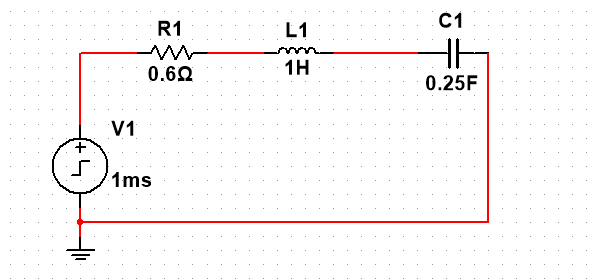
\includegraphics[width=\linewidth]{Report/pics/RLC电路例子.png}
    \caption{Example of RLC circuit. 
    \centering
    \begin{Large}
    $\frac{U_c}{V_1} = \frac{4}{s^2+0.6s+4}$.
    \end{Large}
    }
    \label{fig:RLC circuit example}
  \end{minipage}
  \hfill
  \begin{minipage}[t]{0.5\textwidth}
    \centering
    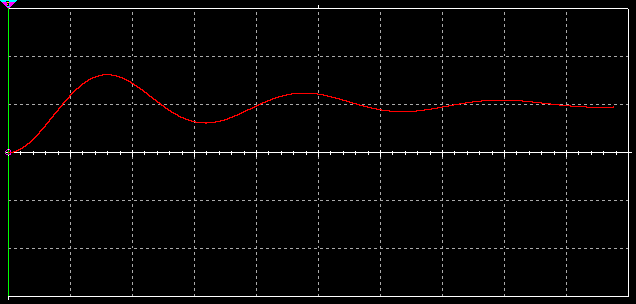
\includegraphics[width=\linewidth]{Report/pics/RLCStepResponse.png}
    \caption{Simulated step response of voltage across capacitor C1. }
    \label{fig:Uc step response}
  \end{minipage}
\end{figure}

A common example which has similar dynamic with the given transfer function is a RLC circuit.

As shown in Fig. \ref{fig:RLC circuit example}, the voltage across the capacitor C1 exhibits dynamic characteristics similar to the given transfer function. Explains are as follows:

\vspace{0.2cm}
Voltage equation of the entire circuit in time domain:
\begin{equation}
    V_1 = U_R+U_L+U_C = R\times I+L\times \frac{dI}{dt}+\frac{1}{C}\int_0^t Idt
    \label{equ:VoltageInTimeDomain}
\end{equation}

Apply Laplacian transform on equation (\ref{equ:VoltageInTimeDomain}), and we have:
\begin{equation}
        V_1(s) = RI(s)+ LI(s)s+\frac{I(s)}{Cs}
        \label{equ:VoltageInSDomain}
\end{equation}

And from equation (\ref{equ:VoltageInSDomain}), the relation of voltage across the capacitor and the source is:
\begin{equation}
    \frac{U_C(s)}{V_1(s)}=\frac{1}{LCs^2+CRs+1}
\end{equation}

Which have similar dynamic with the theoretical plant provided. The simulated step response of voltage across capacitor C1 is shown in Fig. \ref{fig:Uc step response}.

\pagebreak

\section{Control System Block Diagrams}
\textbf{Question:}
\begin{quote}
    Draw two equivalent control system block diagrams, which features the output feedback and the state feedback respectively. Compare the similarity and difference. 
\end{quote}
\textbf{Answer:}

\begin{figure}[htbp]
    \centering
    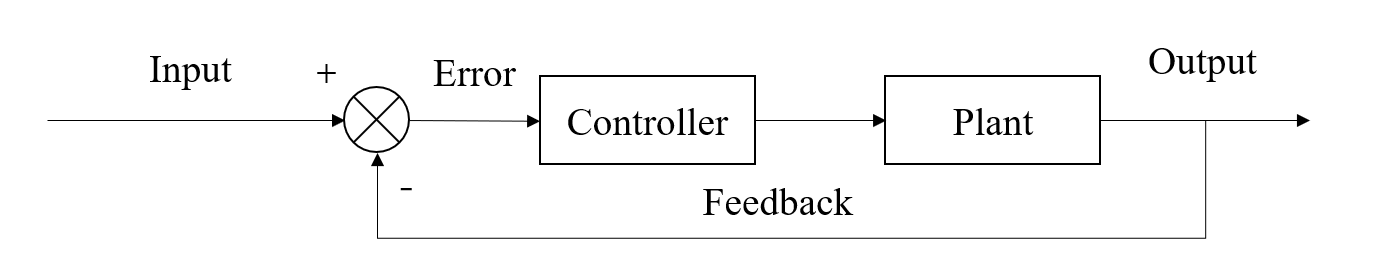
\includegraphics[height = 0.07\paperheight]{Report/pics/OutputFeedbackDiagram.png}
    \caption{Output feedback control diagram.}
    \label{fig:my_label}
\end{figure}

\begin{figure}[htbp]
    \centering
    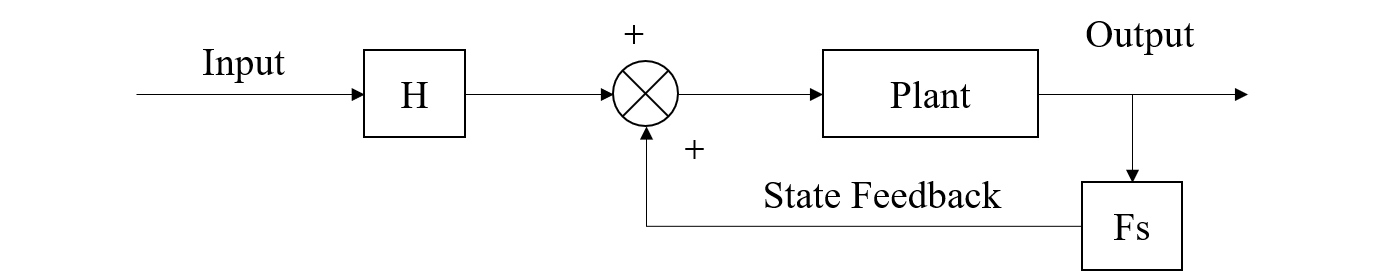
\includegraphics[height = 0.1\paperheight]{Report/pics/StateFeedbackDiagram.png}
    \caption{State feedback control diagram.}
    \label{fig:my_label}
\end{figure}


\textbf{Similarity}
\begin{itemize}
    \item Both methods are used to modify the performance of the system to achieve the desired outcome.
    \item Both methods are closed loop control and using feedback to accomplish the objective of control.
    \item Both methods using linear controlling techniques like poles placing, etc.
\end{itemize}

\textbf{Difference}
\begin{itemize}
    \item State feedback cannot apply to systems whose models are unknown, while the output feedback requires the output only.
    \item The core idea is different: output feedback aims to eliminate/minimize errors, but state feedback is about changing the plant characteristics and creating an ideal system which including the plant as a subsystem.
    \item Output feedback is actually a kind of partially state feedback, for output is a combination of the states. But not all states could be found in output, so the freedom and performance of output feedback is lesser than state feedback.
    \item Output feedback is more suitable for systems that are uncertain and have disturbance.
    \item State feedback is more suitable for systems that are fully examined and have less disturbance.
\end{itemize}



\section{Plant Analyse}
\label{section:plant analyse}
\textbf{Question:}

\begin{quote}    
Analyse the plant performance such stability, observability, controllability, and time response to a unit step reference input.
\end{quote}
\textbf{Answer:}
\begin{itemize}
    \item \textbf{Stability:}
    Poles of the plant are: $-0.3000\pm1.9774i$, both of them are on the left-half of the s-plane, which means that the system is stable.
    \item \textbf{Observability and controllability:} For linear time-invariant systems, controllability and observability are equivalent in continuous time\cite{ControlandObserve}. The following verification is using the observable realisation\cite{CourseMaterial}:

    \begin{equation}
        \begin{cases}
        \left[\begin{array}{ccc}\dot{x_1}(t)\\
        \dot{x_{2}}(t)\end{array}\right]
        =
        \left[\begin{array}{ccc} 0&-4\\
        1&-0.6\end{array}\right]
        \left[\begin{array}{ccc}x_1(t)\\
        x_2(t)\end{array}\right]
        +
        \left[\begin{array}{ccc}1\\
        0\end{array}\right]
        u(t)
        \\
        \\
        y(t)=
        \left[\begin{array}{ccc}0&1\end{array}\right]
        \left[\begin{array}{ccc}x_1(t)\\
        x_2(t)\end{array}\right]
        \end{cases}
    \end{equation}

    For the realisation above, the criterion matrices P, Q and R are:
    $P = \left[\begin{array}{ccc}1&0\\
        0&1\end{array}\right]$, $Q = \left[\begin{array}{ccc}0&1\end{array}\right]$, $R=\left[\begin{array}{ccc}0&1\\
        1&-0.6\end{array}\right]$. It's controllable ($rank(P)=2=n, rank(Q)=1=l$) and observable ($rank(R)=2=n$).

    
    \item \textbf{Unit step response:} 
    \\The unit step response in time domain is as shown in Fig. \ref{fig:PlantStepResponse}. This plant has a slow response speed and steady-state error.
    \vspace{0.3cm}
    \\The mathematical analysis of the unit step response:
    \\When the initial state $x(t_0)=0$, the state transition matrix could be simplified to\cite{CourseMaterial}:
    \begin{equation}
        \phi(t,0)=e^{At}=L^{-1}[(sI-A)^{-1}]=L^{-1}
        \left[\begin{array}{ccc}\frac{5s+3}{5s^2+3s+20}&\frac{-20}{5s^2+3s+20}\\
        \frac{5}{5s^2+3s+20}&\frac{5s}{5s^2+3s+20}\end{array}\right]
    \end{equation}
    And the forced state response could be simplified to:
    \begin{equation}
    \begin{aligned}
        x(t)&=\int_{t_0}^t\phi(t-\tau)Bu(\tau)d\tau+Du(t)\\
        & \approx
        \left[
        \begin{array}{cc}
        0.4830e^{(-0.3t)}sin(1.9774t)-0.15e^{(-0.3t)}cos(1.9774t)+0.15  \\
             0.25-0.0126e^{-0.3t}(19.7737cos(1.9774t)+3sin(1.9774t)) 
        \end{array}
        \right]
    \end{aligned}
    \end{equation}

    Therefore, the output response could be simplified to:
    \begin{equation}
    \begin{aligned}
        y(t)&=Cx(t)+Du(t)\\
        & \approx
        0.25 - 0.0126e^{-0.3t}(19.7737cos(1.9774t) + 3.0sin(1.9774t))
    \end{aligned}
    \end{equation}
    


        \begin{figure}[htbp]
          \centering
          \subfigure[Simulated step response in Simulink.\label{fig:PlantStepResponse}]{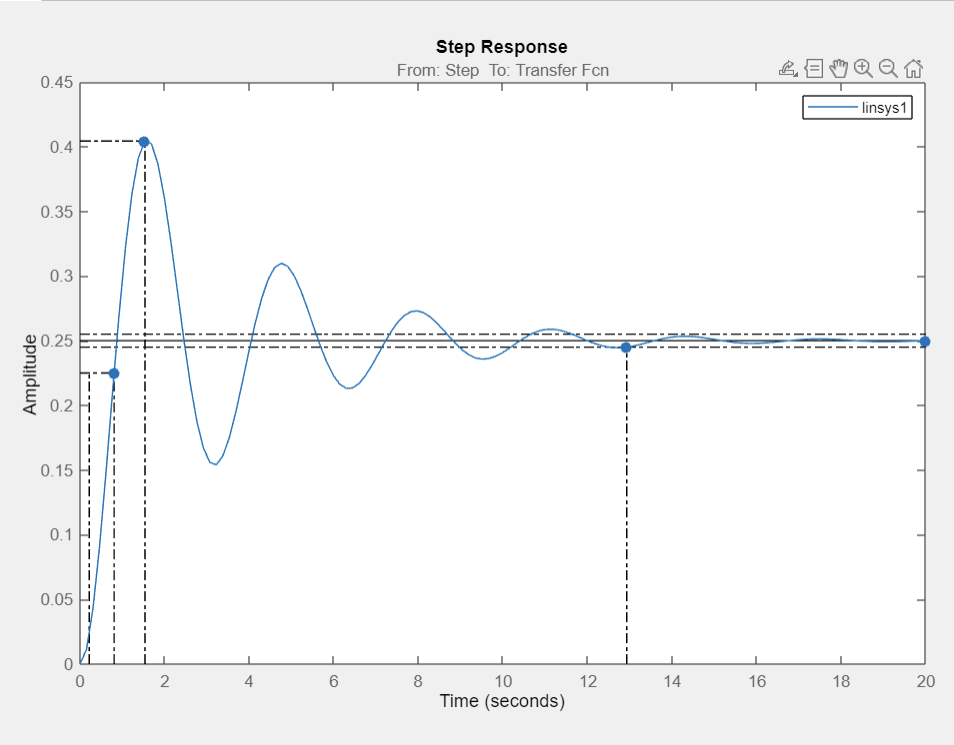
\includegraphics[width=0.45\textwidth]{Report/pics/PlantStepResponse2.png}}
          \quad % or \hfill
          \subfigure[Step response calculated with state transition matrix.\label{fig:SimulatedStepResponse} ]{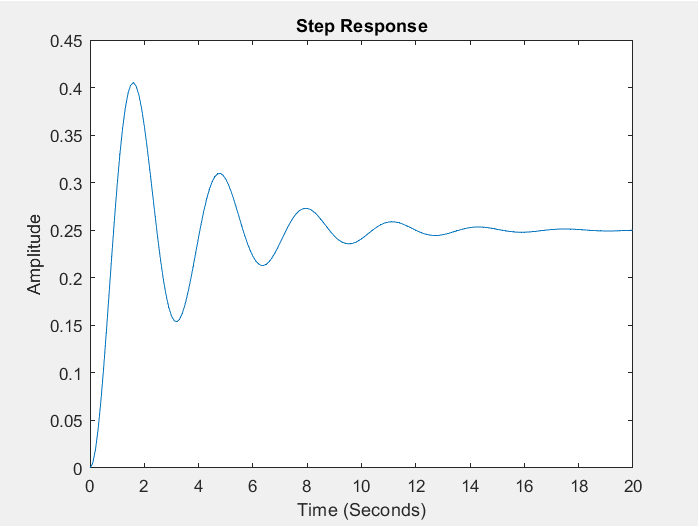
\includegraphics[width=0.45\textwidth]{Report/pics/PlantMathsResponse.png}}
          \caption{Simulated step responses.}
        \end{figure}

    \item \textbf{Other Metrics:}  Other common metrics for second order system performance evaluation:
        \begin{itemize}
            \item Overshoot: 61.7\%
            \item Final value: 0.25
            \item Rise time: 0.588 s
            \item Peak time: 1.54 s
            \item Settling time: 9.83 s (error $\leq$ 5\%)
        \end{itemize}
\end{itemize}



\section{State Feedback Controller Design}
\textbf{Question:}
\begin{quote}
Design a state feedback controller (you specify the reasonable design criteria).
\end{quote}
\textbf{Answer:}


 \textbf{Damping ratio $\xi$ :} Choose the optimal damping ratio $\xi=0.707$\cite{OptimalDampingRatio}. This optimal damping ratio can minimize the cumulative error and its rate of change, but it will cause overshoot for it is in the range of underdamping. Some system may doesn't allow any overshoot, but here in this report we assume the system could tolerate overshoot, for there is no actual system provided. To prevent overshoot from happening, just turn up the damping ratio and make the $\xi \ge 1$.
 
 \textbf{Undamped natural frequency $\omega_n$:} Assuming we need to achieve a settling time (5\% error) of 0.5 seconds, the natural frequency of oscillation would be: $\omega_n = 0.5\times\frac{\xi}{3}=6\sqrt{2}.$

 \textbf{Closed loop denominator}: $s^2+2\xi\omega_{n}s+\omega_{n}^2 \rightarrow s^2+12s+72$.

The form of state feedback controller is\cite{CourseMaterial}:

\begin{equation}
    u(t) = F_{s}x(t)+Hv(t)
\end{equation}

 From the closed loop denominator and steady state final value, we have:

\begin{equation}
    \begin{cases}
        \overline{F}_s = A+BF_s\\
        det\left[sI-\overline{F}_s\right] = s^2+12s+72\\
        H = \left\{ \left[C+DF_s\right]\left[sI-\overline{F}_s\right]^{-1}B+D \right\}_{s=0}^{-1} = \left\{ \left[C+DF_s\right]\left[\overline{F}_s\right]^{-1}B-D \right\}^{-1}
    \end{cases}
    \label{equ:StateFeedbackPrinciple}
\end{equation}

And the solution to Equation (\ref{equ:StateFeedbackPrinciple}) is:
 
 \begin{equation}
     \begin{cases}
         F_s = \left[\begin{array}{ccc}-\frac{57}{5}&-\frac{1529}{25}\end{array}\right]\approx\left[\begin{array}{ccc}-11.4&-61.16\end{array}\right]\\
         H=72
     \end{cases}
 \end{equation}

For the implementation with state observer, please see Section \ref{Performance Simulation}.


\section{Observer Design}
\textbf{Question:}
\begin{quote}
Design a corresponding observer and explain when it will be used. 
\end{quote}
\textbf{Answer:}


\textbf{Observer poles specification:} In general, the response of the state observer should be 2 $\sim$ 5 times faster than the original system\cite{CourseMaterial}, but if the response is too fast, it may amplify small error signals. So the poles of the observer should be further to the imagine axis than the plant.

According to the plant's poles ($s = -0.3000\pm1.9774i$) previously mentioned in Section \ref{section:plant analyse}, the poles of the observer could be: $s=-1.2, s=-1.3$, which means the characteristic equation for the observer would be: $(s+1.2)(s+1.3)=s^2+2.5s+1.56$.

The form of the state observer is:
\begin{equation}
    \dot{\hat{x}}(t) = L\hat{x}(t)+Mu(t)+Ny(t)
\end{equation}

From the characteristic equation and the request of $e(t) = \hat{x}(t)-Tx(t) \approx 0$ ($T \approx 1$ for observer has negative real poles), we could derive that:
\begin{equation}
    N = 
    \left[\begin{array}{ccc}-2.44\\1.9\end{array}\right]
\end{equation}

and:
\begin{equation}
    L = A-NC = \left[\begin{array}{ccc}0&-1.56\\1&-2.5\end{array}\right], 
    M = B-ND = \left[\begin{array}{ccc}1\\0\end{array}\right]
\end{equation}

For the implementation with state observer, please see Section \ref{Performance Simulation}.

\textbf{Applications or situations of use:}
Generally speaking, state observer is a technique of computing internal state information with the system output \cite{Observer}.

When the state cannot be directly measured (like internal deformation of the building) the observer could be useful for it could derive the state information with only the output. 

\section{Performance Simulation}
\label{Performance Simulation}
\textbf{Question:}
\begin{quote}
    Provide relevant performance data and analysis from your simulated studies.
\end{quote}
\textbf{Answer:}

The system simulated with simulink is as shown below:
\begin{figure}[htbp]
    \centering
    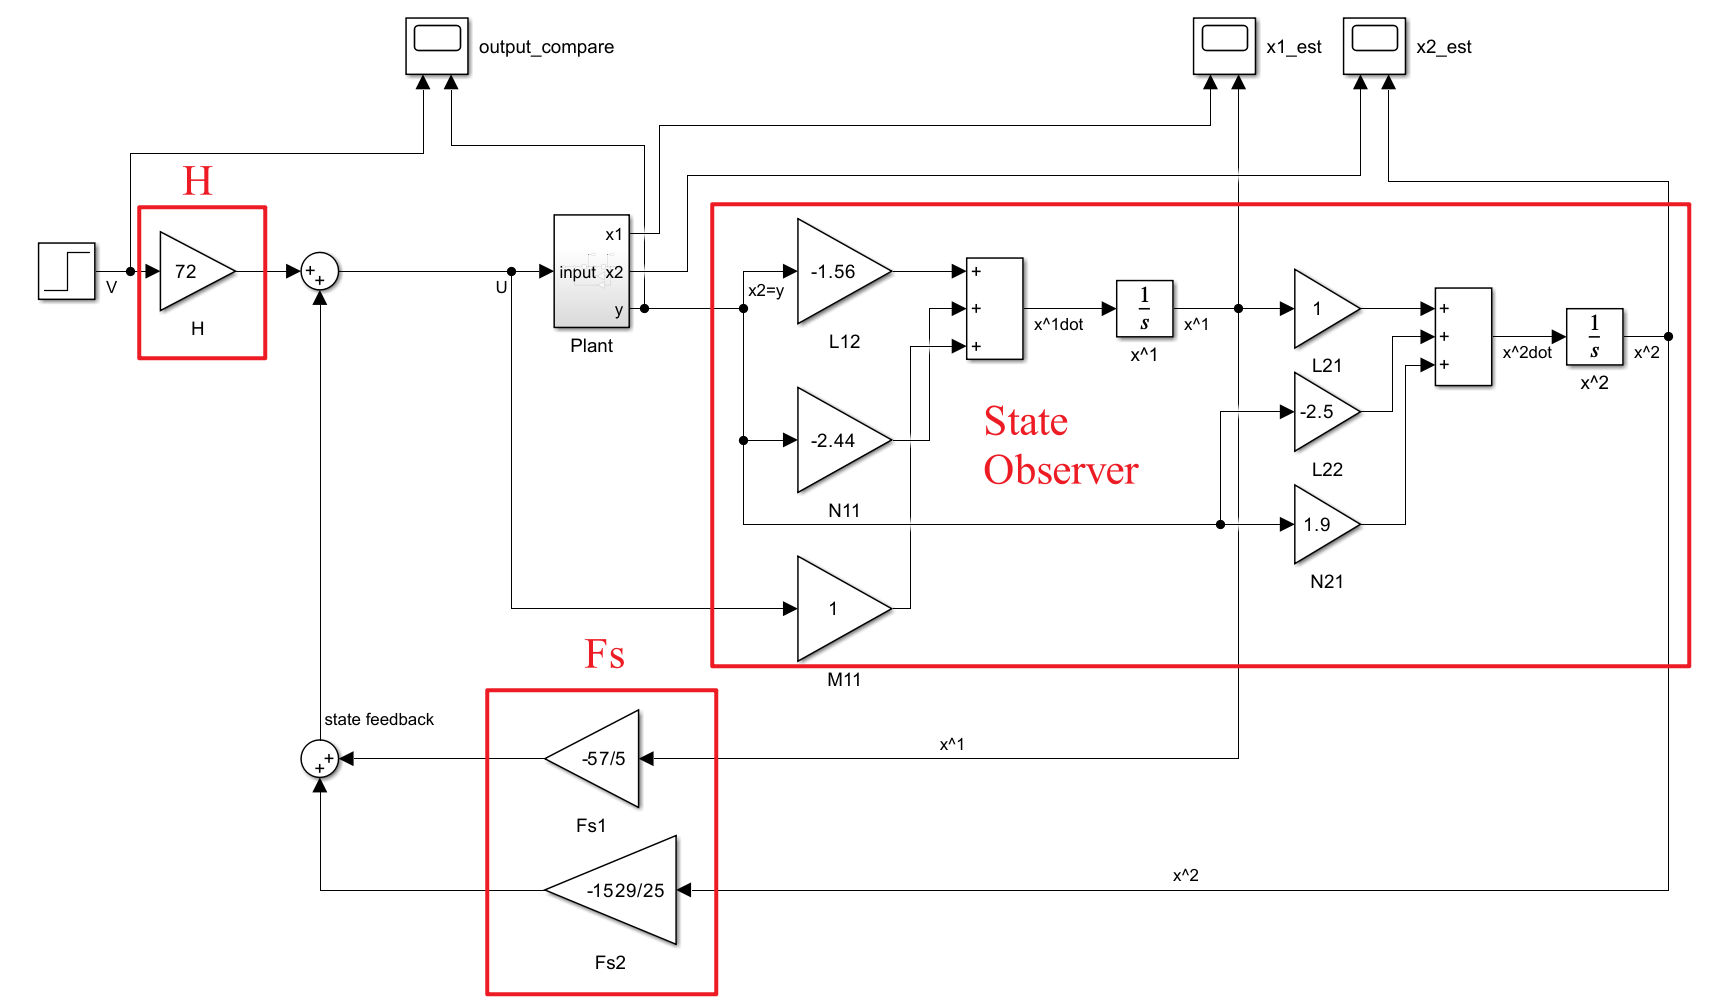
\includegraphics[width = \linewidth]{Report/pics/WholeSystem.png}
    \caption{Overview of the simulated system.}
    \label{fig:WholeSystem}
\end{figure}

\begin{figure}[htbp]
    \centering
    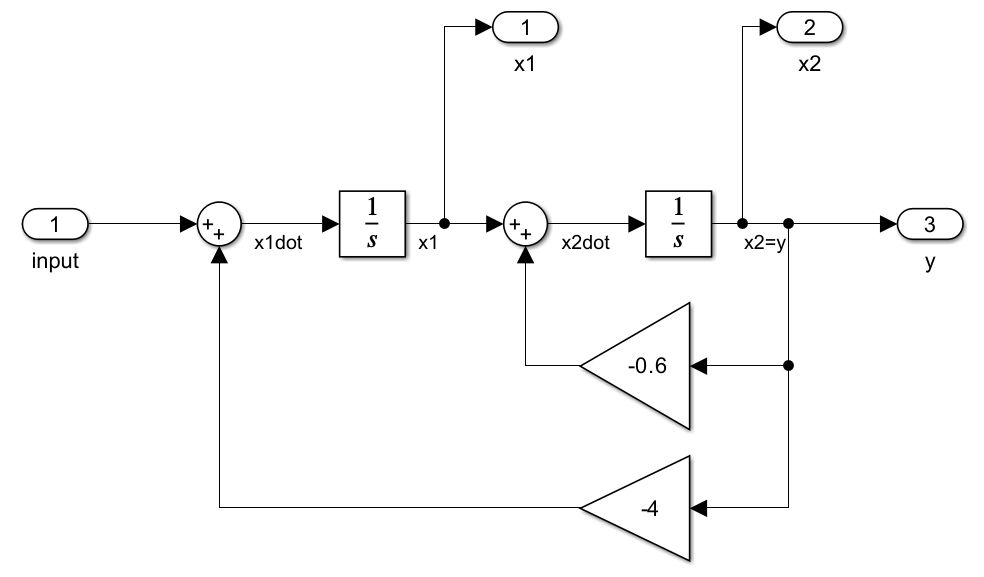
\includegraphics[width=0.9\linewidth]{Report/pics/Plant.png}
    \caption{Simulated plant (subsystem in Fig. \ref{fig:WholeSystem})}
    \label{fig:Plant}
\end{figure}

        \begin{figure}[htbp]
          \centering
          \subfigure[$\hat{x}_1$ from observer and $x_1$ of the plant.\label{fig:Observedx^1}]{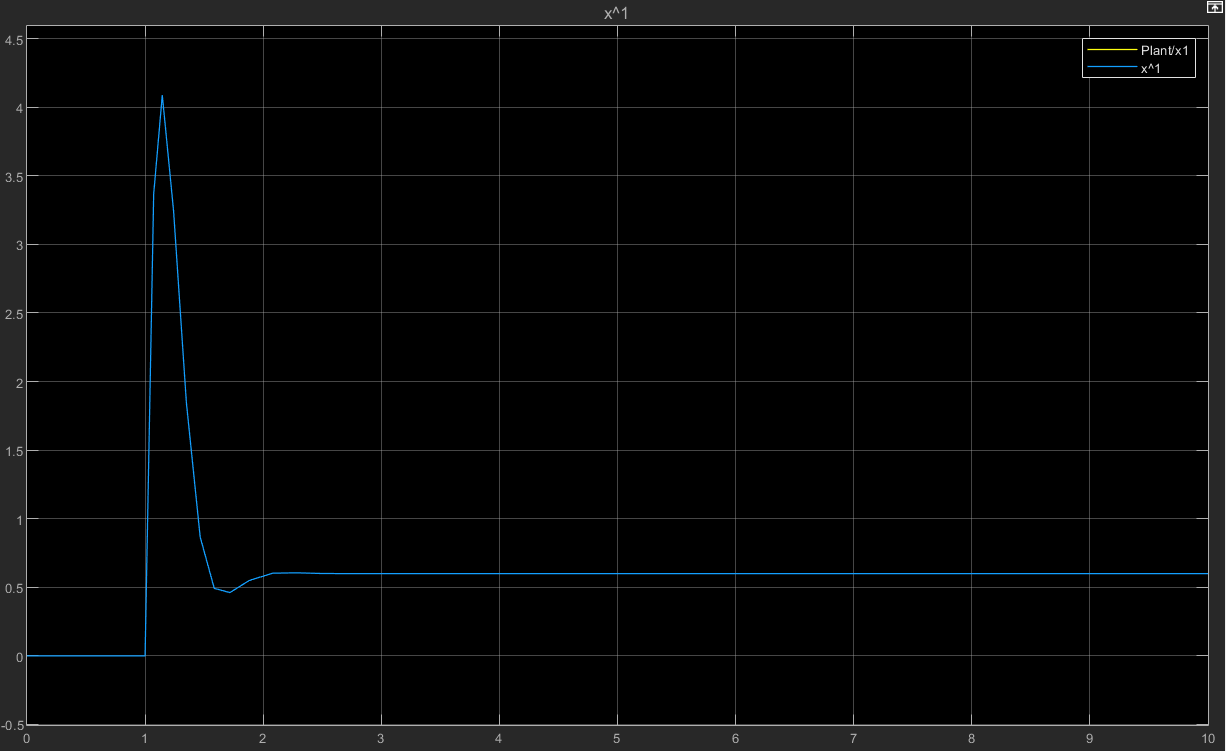
\includegraphics[width=0.8\textwidth]{Report/pics/x^1.png}}
          \hfill%\quad % or \hfill
          \subfigure[$\hat{x}_2$ from observer and $x_2$ of the plant.\label{fig:Observedx^2} ]{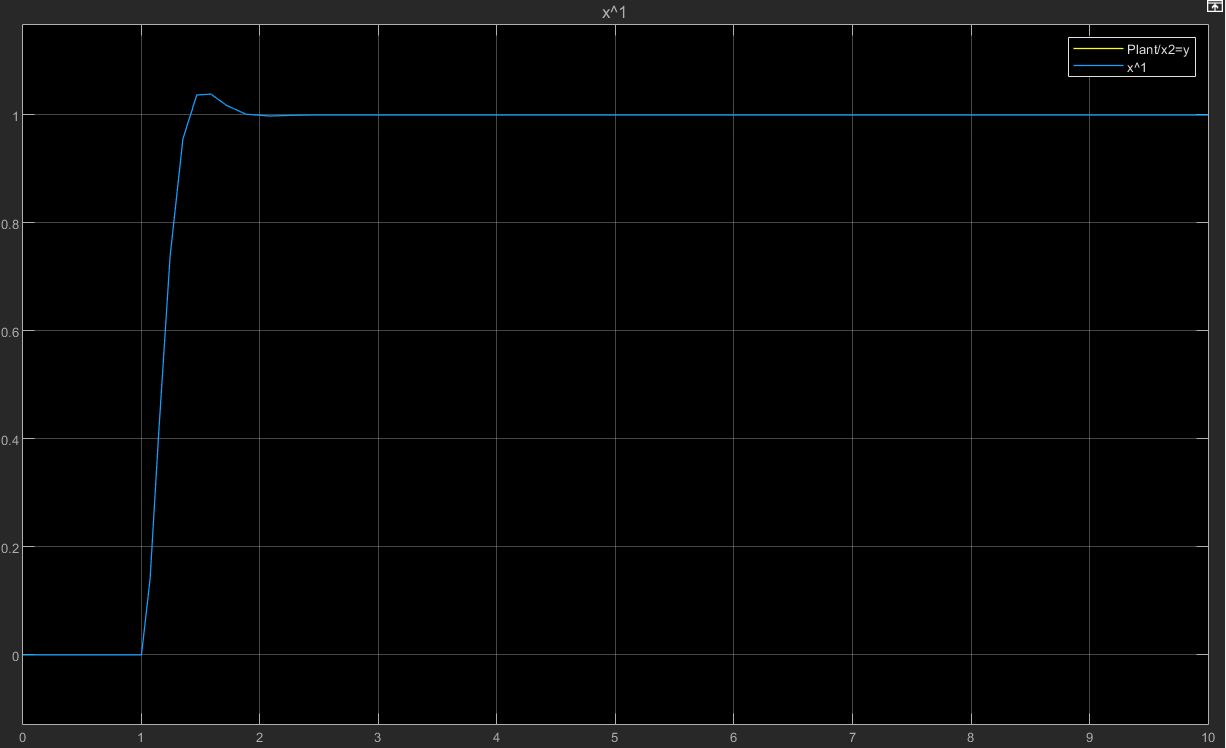
\includegraphics[width=0.8\textwidth]{Report/pics/x^2.png}}
          \caption{Simulated observer results. There is no noticeable errors.}
        \end{figure}

\begin{figure}[htbp]
    \centering
    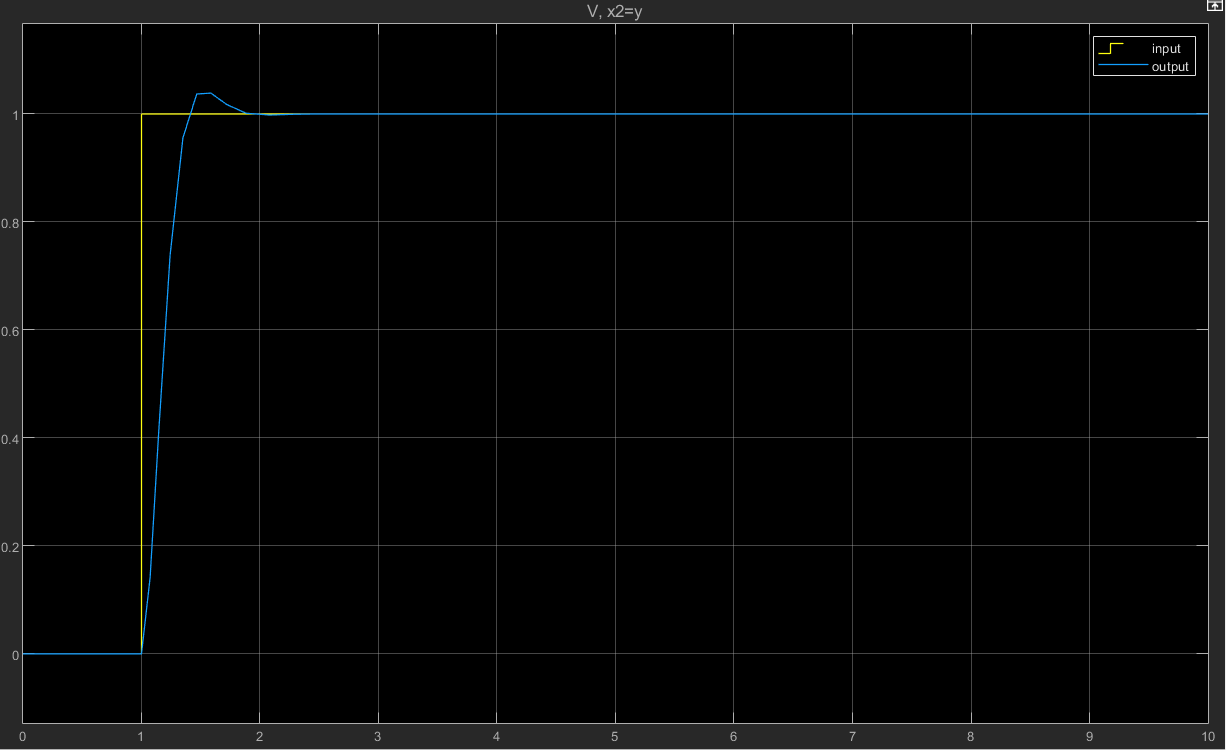
\includegraphics[width = \linewidth]{Report/pics/OutputResult1.png}
    \caption{System output and input (unit step response).}
    \label{fig:OutputResult1}
\end{figure}

\begin{figure}[htbp]
    \centering
    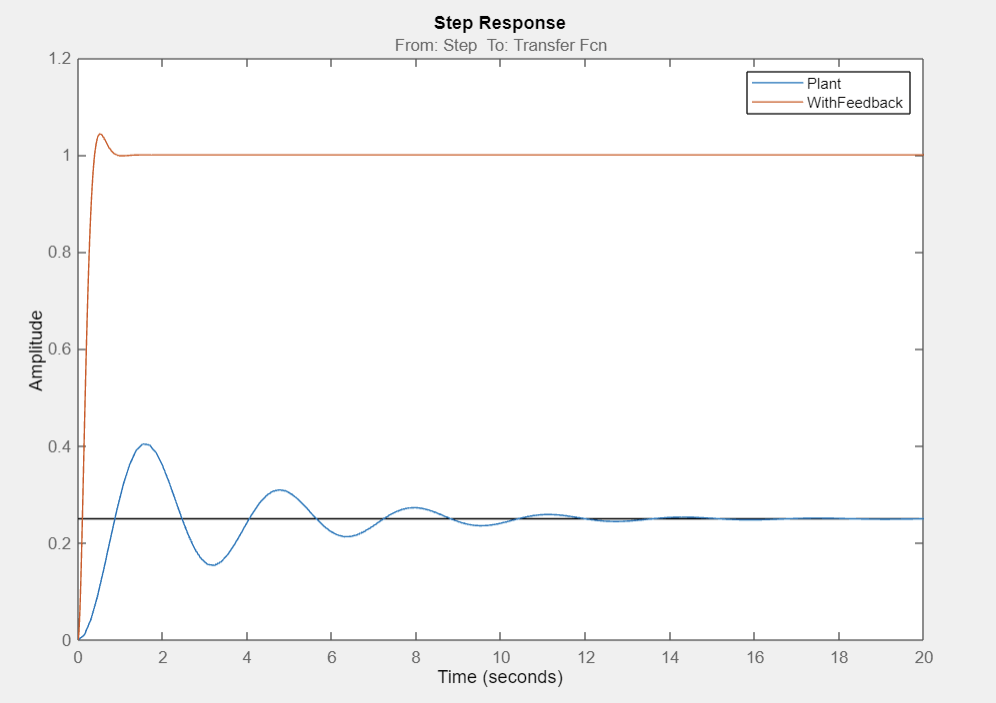
\includegraphics[width=\linewidth]{Report/pics/Compare.png}
    \caption{Comparison of the plant and plant with designed state feedback controller.}
    \label{fig:my_label}
\end{figure}


\FloatBarrier

\textbf{Metrics in time domain:}
\begin{itemize}
            \item Overshoot: 4.000\%
            \item Final value: 1.000
            \item Rise time: 0.313 s
            \item Peak time: 0.522 s
            \item Settling time: 0.522 s (error $\leq$ 5\%)
\end{itemize}

\textbf{Frequency Domain Characteristics:}
\begin{figure}[htbp]
    \centering
    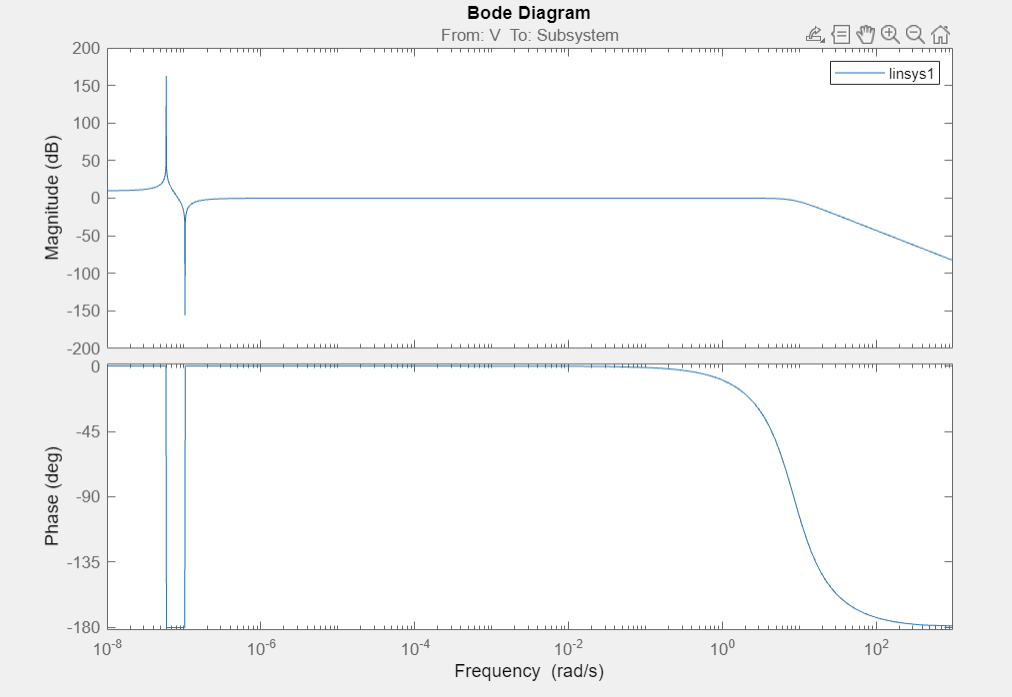
\includegraphics[width=0.6\linewidth]{Report/pics/SystemBode.png}
    \caption{System Bode Diagram.}
    \label{fig:BodeDiagram}
\end{figure}
        
\section{Digital Controller Implementation}
\textbf{Question:}
\begin{quote}
    Discuss the implementation of computer based digital control system including digital controller algorithm and major hardware components. Indicate how you would choose the sampling time required for the computer control system.
\end{quote}
\textbf{Answer:}
The system primarily requires the following components:
\begin{itemize}
    \item \textbf{A/D Converter and D/A Converter:} Convert the system output to digital signal, and convert digital controlling signals to analog values. The choice of A/D, D/A converter model should be mainly based on the channel bandwidth, output range of the system, and the required resolution (which is determined by the error requirements).
    \item \textbf{Sampler/Holder:} Generally, a zero-order hold sampler is sufficient because it is not overly sensitive to noise signals. 
    
    The sampling rate could be determined by the plant's dynamic characteristic: sampling interval must be five or ten times faster than the smallest time constant of the system.\cite{CourseMaterial}

    To determine the time constant, we need to investigate the closed loop poles. A complex pole $\sigma\pm\j\omega$ represents a signal with the form of $Ae^{-\sigma t}sin(\omega t+\phi)$ in time domain. Which means the real part of the pole determines the decaying speed, and the imagine part determines the oscillation frequency.
    
    Poles of the plant are: $s=-0.3000\pm0.19774i$, and the real part of the poles determines the decaying speed of the system. So both of the time constants are $\frac{1}{0.3000}\approx3.3333$.

    And for sampling interval $T$: $T$ could be selected in the interval of $(0.2\sim0.1)*3.3333$, the faster the better. But the sampling rate is also limited by the other factors from other parts of the system like channel bandwidth, processing speed, power supply, and budget.

    Another factor that affects the sampling rate is the desired performance. Slow sampling rate could result in slow responding, deteriorated overshoot and oscillation, etc.
    
    \item \textbf{Logic Circuits:} The operations of the control system designed in this report can be implemented with only basic digital circuit components (op-amp, capacitor, resister, inductance, etc), and in many occasions, these computing may be performed by a micro-controller. The selection of devices in this section should be based on budget considerations.

    In the given system, $x_2=y$ (see Section \ref{section:plant analyse}), so the observer in continuous domain could be simplified as below:
    \begin{equation}
        \begin{cases}
            \hat{\dot{x}}_1 = u-4y\\
            \hat{\dot{x}}_2 = \hat{x}_1-0.6y
        \end{cases}
    \end{equation}
    And the state feedback is:
    \begin{equation}
        u(t) = F_s\hat{x}(t)+Hv(t) = -11.4 \hat{x}_1-61.16 \hat{x}_2+72v
    \end{equation}
    Then, the computing process is:
    \begin{enumerate}
        \item $\hat{\dot{x}}_1$: $\hat{\dot{x}}_1 = u-4y$. 
        \item $\hat{x}_1$: Perform integration  in discrete domain to get $\hat{x}_1$: $\hat{x}_1(t) = \hat{x}_1(t-1)+T*\hat{\dot{x}}_1(t-1)$. $T$ is the sampling interval.
        \item $\hat{\dot{x}}_2$:  $\hat{\dot{x}}_2 = \hat{x}_1-0.6y$. 
        \item $\hat{x}_2$: Perform integration  in discrete domain to get $\hat{x}_2$: $\hat{x}_2(t) = \hat{x}_2(t-1)+T*\hat{\dot{x}}_2(t-1)$. $T$ is the sampling interval.
        \item Calculate the state feedback controlling signal $u$: $u(t) = F_s\hat{x}(t)+Hv(t) = -11.4 \hat{x}_1-61.16 \hat{x}_2+72v$, $v$ is the input signal.
    \end{enumerate}
    
\end{itemize}

\begin{figure}[htbp]
    \centering
    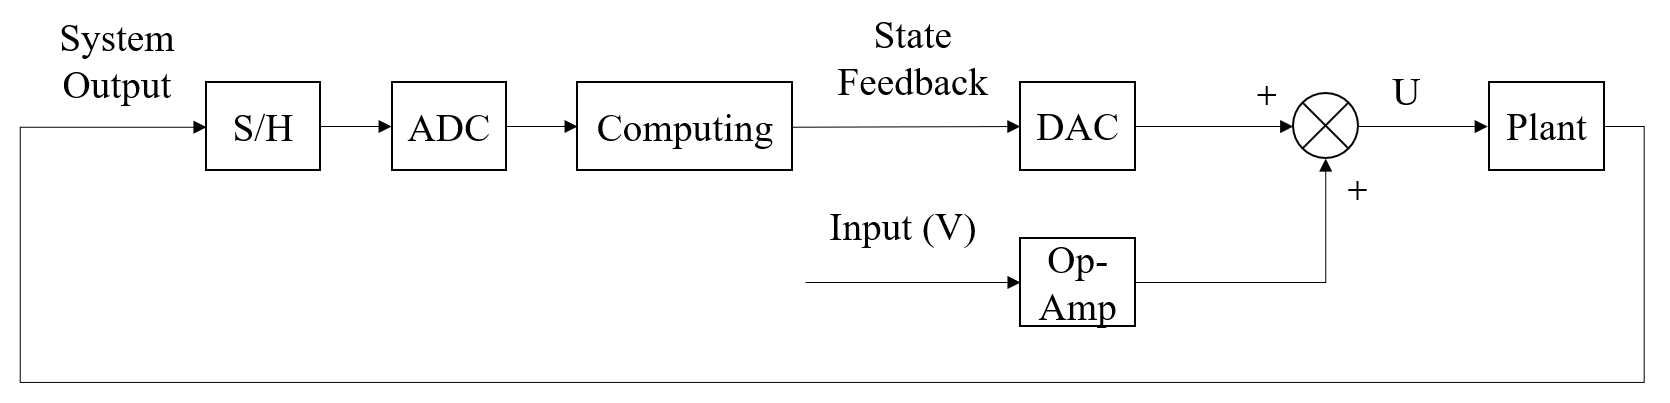
\includegraphics[width = \linewidth]{Report/pics/DigitalDesign.png}
    \caption{Digital controller diagram.}
    \label{fig:my_label}
\end{figure}
\FloatBarrier

\patchcmd{\thebibliography}{\section*{\refname}}{}{}{}

\section{References}

\bibliographystyle{unsrt}
\bibliography{Report/ref}

\end{document}